\chapter{Theoretische Grundlagen}

Um die Funktionsweise von Augmented Reality (AR) und verwandten Technologien zu verstehen, ist ein grundlegendes Wissen über die zugrunde liegenden Konzepte und Techniken erforderlich. In diesem Kapitel werden die theoretischen Grundlagen der Computer Vision und Computergrafik erläutert, die für die Entwicklung von AR-Anwendungen relevant sind. Dabei wird vor der Fokus vor allem auf die Konzepte gelegt, die eine Relevanz für mobile AR-Anwendungen haben. Dazu gehören die Rekonstruktion von 3D-Szenen, die Kamerakalibrierung, die Sensorik, das Tracking und Rendering von virtuellen Objekten. (\cite{doerner2022virtual})

\section{Dreidimensionale Computergrafik}

In der Computergrafik werden dreidimensionale Objekte, auch als Modelle bezeichnet, durch geometrische und relationale Informationen beschrieben. Diese Objekte bestehen in der Regel aus Polygonen, die durch ihre Eckpunkte (Vertices) definiert sind. Ein Polygon ist eine geschlossene Fläche, die durch das Verbinden der Vertices mit geraden Linien entsteht. Ein 3D-Modell wird in einem kartesischen Koordinatensystem beschrieben, wobei die Positionen der Vertices durch ihre \(x\)-, \(y\)- und \(z\)-Koordinaten angegeben werden. (\cite{kore2018space})

Das einfachste Polygon ist ein Dreieck, das nur drei Eckpunkte benötigt. Dreiecke sind planar und konvex, was sie ideal für Berechnungen in der Computergrafik macht, wie beispielsweise bei der Beleuchtung oder Kollisionserkennung. Obwohl komplexere Polygone existieren, werden diese oft in Dreiecke zerlegt, da sie von Grafikpipelines effizienter verarbeitet werden können. Solche Modelle bestehen dann aus Dreiecksnetzen (Meshes), die als Arrays von Vertices und Indizes gespeichert werden. (\cite{wikipedia2023polygons})

Virtuelle 3D-Szenen und Objekte werden in einem kartesischen Koordinatensystem beschrieben. Dieses Koordinatensystem wird üblicherweise als Weltkoordinatensystem bezeichnet, in dem die \(x\)-, \(y\)- und \(z\)-Achsen die drei Dimensionen repräsentieren. In einem rechtshändigen Koordinatensystem zeigt die \(x\)-Achse nach rechts, die \(y\)-Achse nach oben und die \(z\)-Achse nach vorne. Die Position eines Objekts im Raum wird oft mithilfe einer Transformationsmatrix beschrieben. (\cite{appledevdoc, usau2023appleARCamera})

\section{Matrixalgebra}

Das Anwenden von mathematischen Operationen auf Matrizen ist ein grundlegendes Konzept für viele Algorithmen in der Computer Vision. Diese Arbeit setzt voraus, dass der Leser mit den Grundladen der Matrixalgebra vertraut ist. Im Folgenden werden dennoch die wichtigsten Operationen und Konzepte anhand der Transformationen in der Computergrafik erläutert.

Unter der Transformation eines Objektes in einer 3D-Szene versteht man das Verschieben, Drehen oder Skalieren dieses Objektes. Diese Vorgänge können durch Transformationsmatrizen beschrieben werden, die einheitlich auf alle Vertices eines Objekts angewendet werden. Solche Matrizen haben typischerweise die Größe \(4 \times 4\) und kombinieren Translation, Rotation und Skalierung. Dies hat den Vorteil, dass alle Transformationen in einer einzigen Matrix zusammengefasst werden können, was die Berechnungen effizienter macht. (\cite{jazz2020transformMatrix, pezzi2021matrices, freescale2010math3d})

\subsection{Translation}

Die Translation verschiebt ein Objekt entlang der \(x\)-, \(y\)- oder \(z\)-Achse. Die Transformationsmatrix für eine Translation ist wie folgt definiert:

\begin{equation}
\begin{bmatrix}
x' \\ y' \\ z' \\ 1
\end{bmatrix}
=
\begin{bmatrix}
1 & 0 & 0 & t_x \\
0 & 1 & 0 & t_y \\
0 & 0 & 1 & t_z \\
0 & 0 & 0 & 1
\end{bmatrix}
\begin{bmatrix}
x \\ y \\ z \\ 1
\end{bmatrix}
\end{equation}

Hierbei verschieben die Parameter \(t_x\), \(t_y\) und \(t_z\) das Objekt entlang der jeweiligen Achsen.

\subsection{Rotation}

Die Rotation eines Objekts erfolgt um eine der drei Achsen. Die Rotationsmatrizen sind für jede Achse wie folgt definiert:

\paragraph{Rotation um die \(x\)-Achse:}
\begin{equation}
\begin{bmatrix}
1 & 0 & 0 & 0 \\
0 & \cos(\alpha) & -\sin(\alpha) & 0 \\
0 & \sin(\alpha) & \cos(\alpha) & 0 \\
0 & 0 & 0 & 1
\end{bmatrix}
\end{equation}

\paragraph{Rotation um die \(y\)-Achse:}
\begin{equation}
\begin{bmatrix}
\cos(\alpha) & 0 & \sin(\alpha) & 0 \\
0 & 1 & 0 & 0 \\
-\sin(\alpha) & 0 & \cos(\alpha) & 0 \\
0 & 0 & 0 & 1
\end{bmatrix}
\end{equation}

\paragraph{Rotation um die \(z\)-Achse:}
\begin{equation}
\begin{bmatrix}
\cos(\alpha) & -\sin(\alpha) & 0 & 0 \\
\sin(\alpha) & \cos(\alpha) & 0 & 0 \\
0 & 0 & 1 & 0 \\
0 & 0 & 0 & 1
\end{bmatrix}
\end{equation}

Die Reihenfolge, in der Rotationen um verschiedene Achsen durchgeführt werden, ist entscheidend, da sie die finale Orientierung und Position des Objektes beeinflussen. Diese Reihenfolge wird durch Euler-Winkel beschrieben.

\subsection{Skalierung}

Die Skalierung verändert die Größe eines Objekts proportional entlang der \(x\)-, \(y\)- und \(z\)-Achsen. Die Skalierungsmatrix ist wie folgt definiert:

\begin{equation}
\begin{bmatrix}
x' \\ y' \\ z' \\ 1
\end{bmatrix}
=
\begin{bmatrix}
s_x & 0 & 0 & 0 \\
0 & s_y & 0 & 0 \\
0 & 0 & s_z & 0 \\
0 & 0 & 0 & 1
\end{bmatrix}
\begin{bmatrix}
x \\ y \\ z \\ 1
\end{bmatrix}
\end{equation}

Hierbei sind \(s_x\), \(s_y\) und \(s_z\) die Skalierungsfaktoren entlang der jeweiligen Achsen.

\subsection{Anwendung der Transformationen}

Die lokalen Koordinaten eines Objekts können mithilfe einer Transformationsmatrix in Weltkoordinaten umgerechnet werden:

\begin{equation}
P_{world} = T_{object} \cdot P_{object}
\end{equation}

Hierbei ist \(T_{object}\) die Transformationsmatrix des Objekts, und \(P_{object}\) sind die lokalen Koordinaten. Das Ergebnis \(P_{world}\) beschreibt die Position des Objekts im Weltkoordinatensystem.

\section{Kalibrierung}\label{Kalibrierung}

Die Kalibrierung ist ein essenzieller Schritt in der Augmented-Reality-Pipeline. Sie dient der Bestimmung der intrinsischen und extrinsischen Kameraparameter, um eine korrekte Transformation von 2D-Bildpunkten in 3D-Weltkoordinaten zu ermöglichen (\cite{mw2024calibration}).

Dabei wird häufig das sogenannte „Pinhole“-Modell verwendet, das die grundlegenden Eigenschaften einer idealisierten Kamera beschreibt (siehe Abbildung \ref{fig:Pinhole}). Dieses Modell basiert auf der Annahme einer Kamera ohne Objektiv, die lediglich eine kleine Blendenöffnung besitzt. Das Licht fällt durch diese Blende und projiziert ein umgekehrtes Abbild der Szene auf die Rückwand der Kamera (\cite{mw2024calibration}).

\begin{figure}
    \centering
    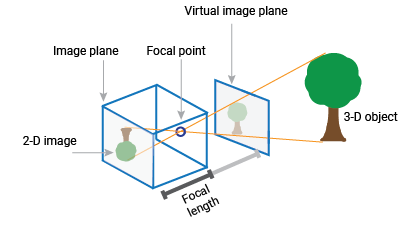
\includegraphics[ width=.5\textwidth ]{pinhole}
    \caption{Pinhole-Modell (\cite{mw2024calibration})\label{fig:Pinhole}}\par
\end{figure}

Mithilfe der intrinsischen und extrinsischen Parameter kann eine Projektionsmatrix bestimmt werden, die es ermöglicht, Bildpixel in das Koordinatensystem der realen Welt zu überführen (siehe Abbildung \ref{fig:Kalibrierung}). Die intrinsischen Parameter umfassen die Brennweite, die Objektivverzerrung und die Position des optischen Zentrums der Kamera. Die extrinsischen Parameter hingegen beschreiben die Position und Orientierung der Kamera im Raum (\cite{mw2024calibration}).

\begin{figure}
    \centering
    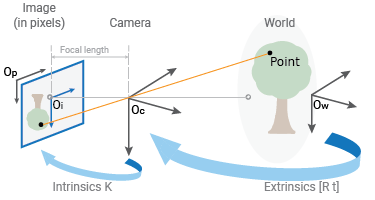
\includegraphics[ width=.5\textwidth ]{calibration-cameramodel-coords}
    \caption{Modell für die Kamerakalibrierung (\cite{mw2024calibration})\label{fig:Kalibrierung}}\par
\end{figure}

Mathematisch wird die Projektionsmatrix \(P\) wie folgt definiert (\cite{mw2024calibration, szeliski2022computerVision}):

\[
P = K[R|t]
\]

Hierbei entspricht \(K\) der intrinsischen Matrix. \(R\) die Rotationsmatrix und \(t\) der Translationsvektor der extrinsischen Matrix. Die intrinsische Matrix \(K\) ist definiert als (\cite{mw2024calibration}):

\[
K = 
\begin{bmatrix}
f_x & s & c_x \\
0 & f_y & c_y \\
0 & 0 & 1
\end{bmatrix}
\]

Hier gilt:

\begin{itemize}
    \item \( f_x \) und \( f_y \): Brennweiten der Kamera in Pixeln, bezogen auf die horizontalen und vertikalen Achsen.
    \item \( c_x \) und \( c_y \): Koordinaten des optischen Zentrums in Pixeln.
    \item \( s \): Skew-Faktor, der berücksichtigt, ob die Kameraachsen orthogonal sind.
\end{itemize}

Die Projektion eines 3D-Punktes \( X = [X, Y, Z, 1]^T \) in das Bildkoordinatensystem \( x = [x, y, 1]^T \) erfolgt dann durch die Gleichung (\cite{mw2024calibration}):

\[
x = PX
\]

Ein Bestandteil der intrinsischen Parameter, das gesondert betrachtet werden muss, sind die Verzerrungen der Linse (engl. Lens-Distortions). Diese entstehen zum einen durch die Krümmung der Linse (Radiale Verzerrzng) und zum anderen durch Unterschiede der Ausrichtung der Linse und des Sensors (Tangentiale Verzerrung). Ohne diese Verzerrungen in die Berechnungen einzubeziehen, kann es Unstimmigkeiten zwischen den berechneten Weltkoordinaten und den realen Weltkoordinaten für einen Bildpunkt geben (\cite{mw2024calibration, szeliski2022computerVision}).

Dazu werden oft Polynommodelle, wie das Brown-Conrady-Modell, verwendet. Dieses Modell relative Position zwischen der Linse und des Sensors. die radiale und tangentialen Verzerrungen der Linse und wird durch die Koeffizienten \( k_1, k_2, k_3 \) und \( p_1, p_2 \) definiert (\cite{brown1966distortion}). Die radiale Verzerrung kann somit durch folgende Gleichung beschrieben werden (\cite{mw2024calibration, szeliski2022computerVision}):

\[
x_{\text{distorted}}   
=
x_{\text{undistorted}}
\left( 1 + k_1 r^2 + k_2 r^4 + k_3 r^6 \right)
\]
\[
y_{\text{distorted}}   
=
y_{\text{undistorted}}
\left( 1 + k_1 r^2 + k_2 r^4 + k_3 r^6 \right)
\]

In diesem Kapitel wurde die Kamera-Kalibrierung anhand einfacher Modelle erläutert. In der Praxis sind die intrinsischen Parameter jedoch in den meisten Kameras bereits vorkalibriert und können von den Herstellern bereitgestellt werden. So integriert beispielsweise Apples ARKit die intrinsischen Kameraparameter direkt und stellt sie über die Klasse \texttt{AVCameraCalibrationData} zur Verfügung, wodurch sie einfach genutzt werden können (\cite{appledevdoc}).

Die extrinsischen Parameter hingegen müssen häufig manuell bestimmt werden, um die exakte Position und Orientierung der Kamera zu ermitteln. In der Augmented Reality ist die präzise Bestimmung der Kameraposition essenziell für viele Tracking-Verfahren. Dabei unterscheidet man zwischen markerbasiertem Tracking (siehe Kapitel \ref{Markerbasiertes Tracking}), bei dem die Position und Größe eines bekannten Markers – oft ein Schachbrettmuster – in der realen Welt genutzt wird, und markerlosem Tracking (siehe Kapitel \ref{SfM} und \ref{SLAM}), bei dem die Kameraposition durch die Analyse von Bilddaten ermittelt wird (\cite{doerner2022virtual, alam2024calibration}).

\section{Sensorik}

Die Erfassung der Umgebung in Augmented-Reality-Anwendungen erfolgt mithilfe verschiedener Sensoren, die Daten über die physische Welt liefern. Je nach Anwendungsfall und Eingabegerät können unterschiedliche Sensoren verwendet werden, um die Position und Bewegung des Geräts zu bestimmen. Bei vielen Tracking-Verfahren werden eine Kombination von Sensoren verwendet, um die Genauigkeit und Zuverlässigkeit der Positionsschätzung zu verbessern. Beispielsweise kann die Kamera für visuelle Tracking-Anwendungen verwendet werden, während das IMU für die Schätzung der Bewegung des Geräts verwendet wird. Durch die Fusion von Daten aus verschiedenen Sensoren können AR-Anwendungen eine präzise und konsistente Darstellung der virtuellen Objekte in der realen Welt erreichen. Die wichtigsten Sensorenarten werden in diesem Abschnitt erläutert.

\subsection{Inertiale Sensoren}

Inertiale Sensoren erfassen die Beschleunigung und Rotation eines Geräts und bestehen typischerweise aus einem Gyroskop und einem Beschleunigungsmesser. Während das Gyroskop die Winkelgeschwindigkeit misst und Drehbewegungen erkennt, erfasst der Beschleunigungsmesser lineare Beschleunigungen. Durch die Kombination beider Sensoren in einer Inertial Measurement Unit (IMU) lassen sich Bewegungen in sechs Freiheitsgraden (3D-Position und -Orientierung) präzise bestimmen. Diese Technologie ist besonders nützlich zur Erfassung schneller Bewegungen und findet Anwendung in AR-Brillen, Smartphones und anderen mobilen Geräten (\cite{doerner2022virtual}).

\begin{tcolorbox}[colback=THAi-Blue!20!white, colframe=THAi-Blue]
    Als \textbf{Freiheitsgrade} (engl. Degrees of Freedom – DOF) werden voneinander unabhängige Bewegungsmöglichkeiten eines physikalischen Systems bezeichnet. Ein starrer Körper besitzt sechs Freiheitsgrade: je drei für die Translation und Rotation. //TODO: Quelle
\end{tcolorbox}
    

\subsection{Kamera}

Die Kamera ist ein essentieller Sensor für AR-Anwendungen, da die visuellen Informationen von vielen Tracking-Verfahren genutzt werden und die aufgenommenen Bilder die Grundlage für die Darstellung von virtuellen Objekten in der realen Welt bilden. Die Kamera liefert Bilddaten, die zur Erkennung von Markern, Features oder Objekten verwendet werden. Durch die Analyse der Kamerabilder können AR-Anwendungen die Position und Orientierung des Geräts bestimmen und virtuelle Objekte in die reale Welt einfügen. (\cite{doerner2022virtual}).

\subsection{Lasersensoren}

Lasersensoren messen die Entfernung zu Objekten mithilfe von Laserstrahlen. LiDAR (Light Detection and Ranging) ist ein bekannter Lasersensor, der in der Robotik, Automobilindustrie und Augmented Reality weit verbreitet ist. Der Sensor strahlt Laserlicht aus und misst die Zeit, die das Licht benötigt, um zu einem Punkt in der Umgebung zu gelangen und zurückzukehren. Dadurch ist die exakte Bestimmung der Position und Entfernung des Punktes zum Sensor möglich. Dies ermöglicht die präzise Erfassung von Tiefeninformationen in der Umgebung und bietet somit große Vorteile für die Genauigkeit und Zuverlässigkeit des Trackings in AR-Anwendungen (\cite{doerner2022virtual}).

\subsection{Satellitengestütze Systeme}

Satellitengestützte Systeme wie GPS (Global Positioning System) bestimmen die geografische Position des Geräts mithilfe von Satellitensignalen. Diese Systeme sind besonders nützlich für die Lokalisierung des Geräts in großen Außenbereichen. Da GPS-Signale jedoch durch Gebäude und andere Hindernisse blockiert werden können, sind sie in Innenräumen oft ungenau. Zusätzlich dazu sind Abweichungen von bis zu 10m möglich, was für viele AR-Anwendungen nicht ausreichend ist. Smartphones setzen daher häufig A-GPS (Assisted GPS) ein um die GPS-Daten mithilfe von Mobilfunknetz- bzw. WLAN-Daten zu präzisieren (\cite{doerner2022virtual}). 

\subsection{Magnetfeldbasierte Sensoren}

Magnetfeldbasierte Sensoren, wie das Magnetometer in IMUs, messen das Magnetfeld der Erde und liefern so Rückschlüsse bezüglich der Orientierung des Geräts relativ zum Magnetfeld. Diese Sensoren sind besonders nützlich für die Bestimmung der Ausrichtung des Geräts im Raum. Allerdings sind Magnetfelder anfällig für Störungen durch elektrische Geräte und Metallgegenstände, was die Genauigkeit der Messungen beeinträchtigen kann. Dennoch sind magnetfeldbasierte Sensoren eine wichtige Ergänzung zu anderen Sensoren für die präzise Lokalisierung und Orientierung in AR-Anwendungen (\cite{doerner2022virtual}).

\section{Markenbasiertes Tracking}\label{Markerbasiertes Tracking}

Das markenbasierte Tracking basiert auf der Erkennung von speziellen Markern, die in der realen Welt platziert sind. Diese Marker dienen als Referenzpunkte für die Positionierung von virtuellen Objekten dienen und ermöglichen es, die extrinsischen Parameter der Kamera zu bestimmen. Die Marker weisen in der Regel ein eindeutiges Muster auf, das von der Kamera erkannt und verfolgt werden kann. Ebenso sind die Dimensionen des Markers bekannt, was die Bestimmung der Position und Orientierung des Markers im Raum erleichtert. Es gibt eine Reihe von Verfahren die unterschiedliche Marker-Typen verwenden und auf unterschiedliche Art und Weise die Position und Orientierung des Markers bestimmen. Vereinfacht dargestellt, funktioniert das markenbasierte Tracking wie folgt:

\begin{figure}
    \centering
    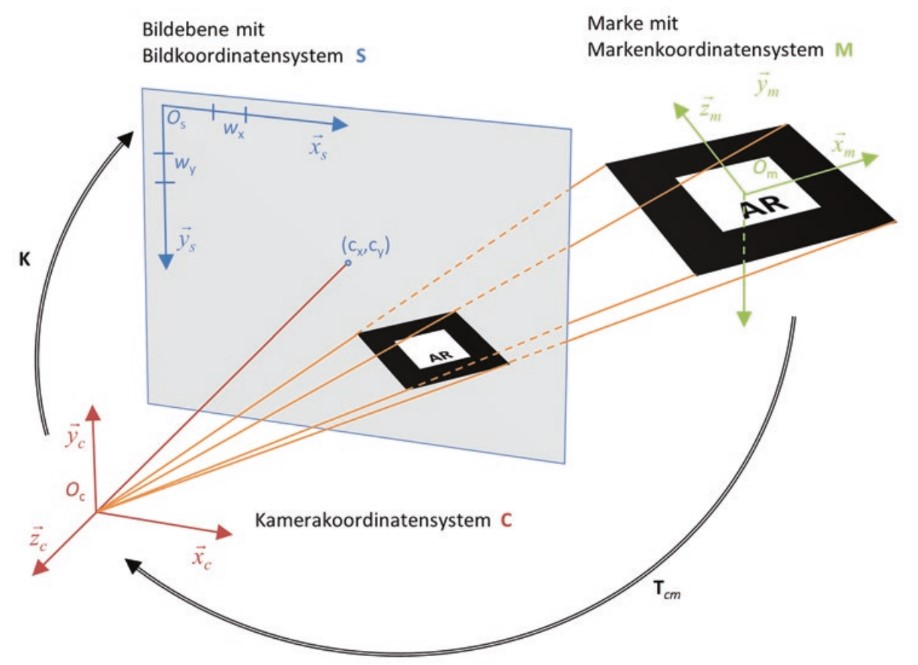
\includegraphics[ width=.5\textwidth ]{Marker}
    \caption{Darstellung eines markenbasiertes Tracking\label{fig:Marker}}\par
\end{figure}

Wie in Abbildung \ref{fig:Marker} dargestellt, wird die Kamera auf den Marker gerichtet, um ihn zu erfassen. Nun kann mithilfe der intrinsischen Kameraparameter und der bekannten Dimensionen des Markers die Position und Orientierung des Kamerakoordinatensystems relativ zum Marker bestimmt werden. Dies ermöglicht die Bestimmung einer Transformationsmatrix \( T_cm \), mithilfe derer die Koordinaten des Markers im Markerkoordinatensystem ins Kamerakoordinatensystem transformiert werden können. Entsprechend der Abbildung \ref{fig:Marker} kann die Transformation \( T_cm \) wie folgt definiert werden:

\begin{equation}\label{eq:v_c}
v_c = T_cm * v_m
\end{equation}

Wobei \( v_c \) Pixelkoordinaten des Markers im Kamerakoordinatensystem und \( v_m \) Koordinaten im Markerkoordinatensystem entsprechen.

Wobei \( v_c \) Pixelkoordinaten des Markers im Kamerakoordinatensystem und \( v_m \) Koordinaten im Markerkoordinatensystem entrsprechen.

Nun können Koordinaten \( v_s \) im Bildkoordinatensystem \( C \) mithilfe der intrinsischen Kameraparameter (siehe Kapitel \ref{Kalibrierung}) und Koordinaten \( v_c \) im Kamerakoordinatensystem wie folgt beschrieben werden:

\[ v_s = K * v_c \]

Unter Verwendung der Gleichung \ref{eq:v_c} kann die Transformation \( T_cm \) in die Gleichung eingesetzt werden:

\[ v_s = K * T_cm * v_m \]

Da \(v_s\) und \(v_m\) bekannt sind (die Pixelkoordinaten des Markers und die bekannten Dimensionen des Markers), kann die Transformation \(T_cm\) berechnet werden.

Die Position und Orientierung des Markers im Raum sind somit bekannt und können zur Platzierung von virtuellen Objekten verwendet werden (\cite{doerner2022virtual}).

Das markerbasierte Tracking ist besonders robust und präzise, da die Position und Orientierung des Markers bekannt sind. Allerdings ist es auch aufwendiger, da die Marker manuell platziert und kalibriert werden müssen. Es wird häufig in Anwendungen eingesetzt, bei denen die Position des darzustellenden Objekts genau bekannt ist. Auch in der Filmproduktion wird markerbasiertes Tracking oft für Motion-Caputre-Verfahren verwendet.

\section{Structure from Motion}\label{SfM}

Structure from Motion (SfM) ist eine Technik aus der Computer Vision, die verwendet wird, um die 3D-Struktur einer Szene aus einer Reihe von 2D-Bildern zu rekonstruieren. SfM basiert auf der Triangulation von Punkten, die in verschiedenen Bildern sichtbar sind, um die Positionen der Sensoren und der Punkte in der Szene zu bestimmen.

Da SfM die Grundlage vieler AR-Verfahren darstellt und in verbesserter bzw. abgewandelter Form in vielen AR-Frameworks (z.B. SLAM, siehe Kapitel 4.7) eingesetzt wird, ist es wichtig, die grundlegenden Schritte und Algorithmen zu verstehen, die bei der Rekonstruktion von 3D-Szenen verwendet werden. Diese werden im Folgenden erläutert.

\subsection{Feature Detection und Matching}

Bei der Feature Detection bzw. beim Feature Maching werden Merkmale in verschiedenen Bildern identifiziert und korrespondierende Merkmale gefunden. Dieser Schritt ist entscheidend, um die Bewegung der Kamera (Tracking) und die 3D-Struktur der Szene zu bestimmen. Es gibt verschiedene Algorithmen, die für das Erkennen und Nachverfolgen von Feature-Punkten verwendet werden können, wie z. B. SIFT (Scale-Invariant Feature Transform), SURF (Speeded-Up Robust Features) oder ORB (Oriented FAST and Rotated BRIEF). Diese Algorithmen setzen sich grundsätzlich aus drei Teilen zusammen:

\begin{enumerate}
    \item Feature Detector oder Keypoint Detector
    \item Feature Descriptor
    \item Feature Matching Algorithm
\end{enumerate}

Der Feature Detector identifiziert charakteristische Punkte im Bild, die sich durch hohe Kontraste oder markante Strukturen auszeichnen. Diese Punkte, auch als Keypoints bezeichnet, dienen als Referenz für spätere Berechnungen. Anschließend erstellt der Feature Descriptor eine numerische Beschreibung für jedes erkannte Merkmal, um sie über mehrere Bilder hinweg vergleichbar zu machen. Diese Deskriptoren bestehen in der Regel aus Vektoren, die die Helligkeitsverteilung um den jeweiligen Feature-Punkt erfassen. Schließlich vergleicht der Feature Matching Algorithmus die Deskriptoren aus verschiedenen Bildern, um korrespondierende Merkmale zu finden, die wiederum zur Schätzung der Kamerabewegung genutzt werden.

Ein besonders effizienter und robuster Algorithmus ist ORB, der auf den Methoden FAST (Features from Accelerated Segment Test) und BRIEF (Binary Robust Independent Elementary Features) basiert. Der FAST-Algorithmus erkennt Punkte mit starken Helligkeitsänderungen, indem er benachbarte Pixel in einem Kreis um den zu prüfenden Pixel vergleicht. Übersteigt die Anzahl der signifikant helleren oder dunkleren Pixel einen bestimmten Schwellenwert, wird der Punkt als Feature identifiziert. Anschließend berechnet BRIEF für jedes erkannte Feature binäre Deskriptoren, indem zufällig gewählte Pixelpaare innerhalb der Umgebung des Feature-Punkts verglichen werden. Die resultierenden binären Deskriptoren sind besonders effizient in der Berechnung und Speicherung. Um die erkannten Merkmale schnell und zuverlässig zuzuordnen, kommt die Fast Library for Approximate Nearest Neighbors (FLANN) zum Einsatz, die eine leistungsstarke Methode zur Suche nach korrespondierenden Features bietet.

Neben klassischen Verfahren wie ORB gewinnen Deep-Learning-Modelle zunehmend an Bedeutung für das Feature Matching. Besonders Convolutional Neural Networks (CNNs) und Transformer-Modelle liefern vielversprechende Ergebnisse. Ein Beispiel hierfür ist XFeat (Accelerated Features), ein optimiertes neuronales Netzwerk, das die Merkmalsextraktion beschleunigt. Auch OmniGlue, eine Kombination aus CNNs und Transformer-Modellen, setzt neue Maßstäbe in der robusten und anpassungsfähigen Feature-Matching-Strategie. Diese modernen Ansätze bieten oft eine höhere Genauigkeit und Stabilität, insbesondere in komplexen Szenen oder bei stark variierenden Lichtverhältnissen.

\subsection{Camera Pose Estimation}

Die Schätzung der Kameraposition ist ein essenzieller Schritt in der SfM-Pipeline, da sie die Position und Orientierung der Kamera in jedem Bild bestimmt. Diese Informationen sind entscheidend für die Rekonstruktion der 3D-Struktur der Szene und die Bestimmung der extrinsischen Kameraparameter.

Geht man davon aus, dass die intrinsischen Parameter der Kamera bekannt sind und mehrere Bilder mit korrespondierenden Punkten vorliegen, kann die Kameraposition mithilfe der Essential Matrix \(E\) berechnet werden. Diese Matrix beschreibt die geometrische Beziehung zwischen zwei Bildern und ermöglicht die Bestimmung von Rotation und Translation der Kamera. Die grundlegende Bedingung für die Berechnung der extrinsischen Parameter lautet:

\begin{equation}
x'^T E x = 0
\end{equation}

Diese Gleichung beschreibt die Epipolargeometrie, wobei \( x \) und \( x' \) die korrespondierenden Punkte in den beiden Bildern darstellen. Die Essential Matrix kann durch den Five-Point-Algorithmus geschätzt werden, der im kalibrierten Fall mindestens fünf korrespondierende Punkte benötigt, um eine eindeutige Lösung zu liefern.

Sobald die Essential Matrix bestimmt wurde, kann sie mithilfe der Singulärwertzerlegung (SVD) in die Rotationsmatrix \( R \) und die Translationsmatrix \( t \) der Kamera zerlegt werden:

\begin{equation}
E = R [t]_x
\end{equation}

Diese Zerlegung erlaubt es, die Bewegung der Kamera zwischen den Bildern präzise zu bestimmen.

\subsection{Dreidimensionale Rekonstruktion}

Die dreidimensionale Rekonstruktion einer Szene überführt die zweidimensionalen Bilddaten einer Kamera in ein 3D-Modell. Dabei werden sowohl die Kameraparameter als auch die Translation und Rotation der Kamera sowie die korrespondierenden Feature-Punkte aus dem Feature Matching verwendet, um die Positionen der Punkte im Raum zu berechnen und so eine präzise 3D-Darstellung der Szene zu erstellen.

Ein zentraler Schritt in der 3D-Rekonstruktion ist die Triangulation, bei der die kartesischen Koordinaten eines Feature-Punktes im Weltkoordinatensystem ermittelt werden. Ein einfaches Verfahren zur Bestimmung dieser Koordinaten besteht darin, den 3D-Strahlen zu folgen, die von den Kamerazentren \( c_j \) in die Richtungen \( \hat{v_j} \) verlaufen. Der gesuchte Punkt \( p_0 \) ist derjenige, der sich im minimalen Abstand zu allen Strahlen befindet. Die Richtungen \( \hat{v_j} \) werden durch die Transformation der 2D-Bildpunkte mittels der Kameramatrizen beschrieben. Der Punkt \( p_0 \) wird dabei durch Minimierung der quadratischen Abstände zwischen den Strahlen und dem Punkt berechnet.

\begin{figure}
    \centering
    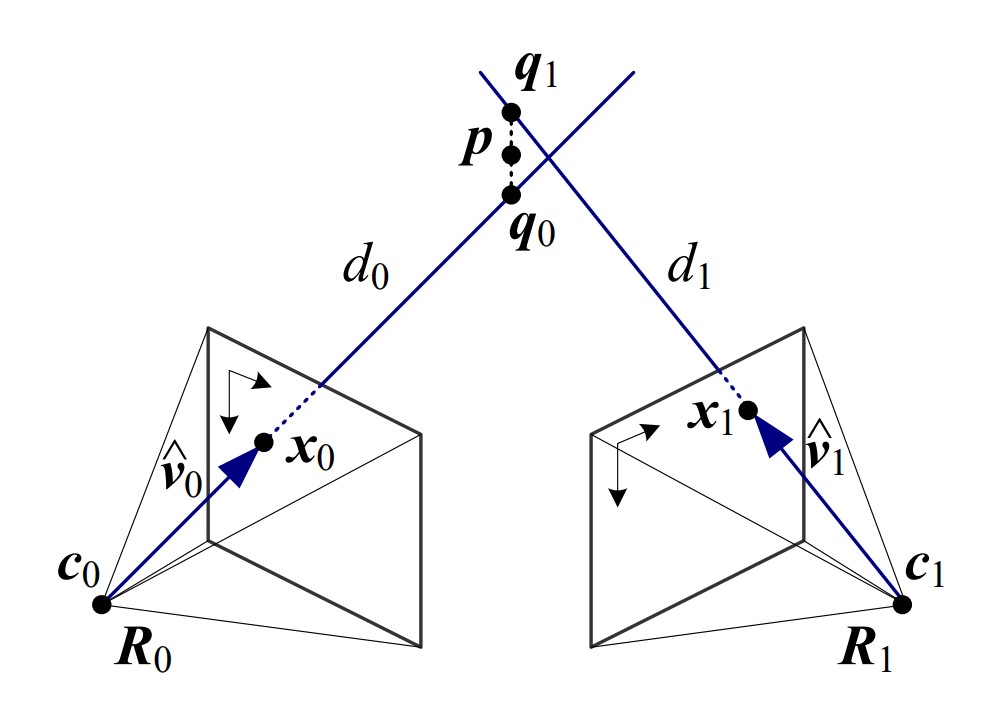
\includegraphics[width=.5\textwidth]{Triangulation}
    \caption{Dreidimensionale Triangulation mit zwei Bildern\label{fig:Triangulation}}\par
\end{figure}

Abbildung \ref{fig:Triangulation} zeigt die grafische Darstellung der Triangulation eines Punktes im dreidimensionalen Raum. Mathematisch wird dieser Prozess durch die folgende Gleichung beschrieben:

\[
p = \left( \sum_j \left( I - \hat{v_j} \hat{v_j}^T \right) \right)^{-1} \left( \sum_j \left( I - \hat{v_j} \hat{v_j}^T \right) c_j \right)
\]

Das Ergebnis der Triangulation ist eine sogenannte Punktwolke (Point Cloud), die die 3D-Struktur der Szene abbildet. Diese Punktwolke kann anschließend weiterverarbeitet werden, um ein detailliertes 3D-Modell der Szene zu erstellen. Ein wichtiger Schritt in dieser Weiterverarbeitung ist die Oberflächenrekonstruktion (Plane Detection), bei der die Punktwolke in Flächen unterteilt wird, um die Oberflächen von Objekten im Raum zu bestimmen. Zur Durchführung der Oberflächenrekonstruktion wird häufig der RANSAC-Algorithmus (Random Sample Consensus) eingesetzt. Dieser Algorithmus erkennt Ausreißer in den Daten und schätzt die Flächen anhand der verbleibenden, konsistenten Punkte.

\begin{figure}
    \centering
    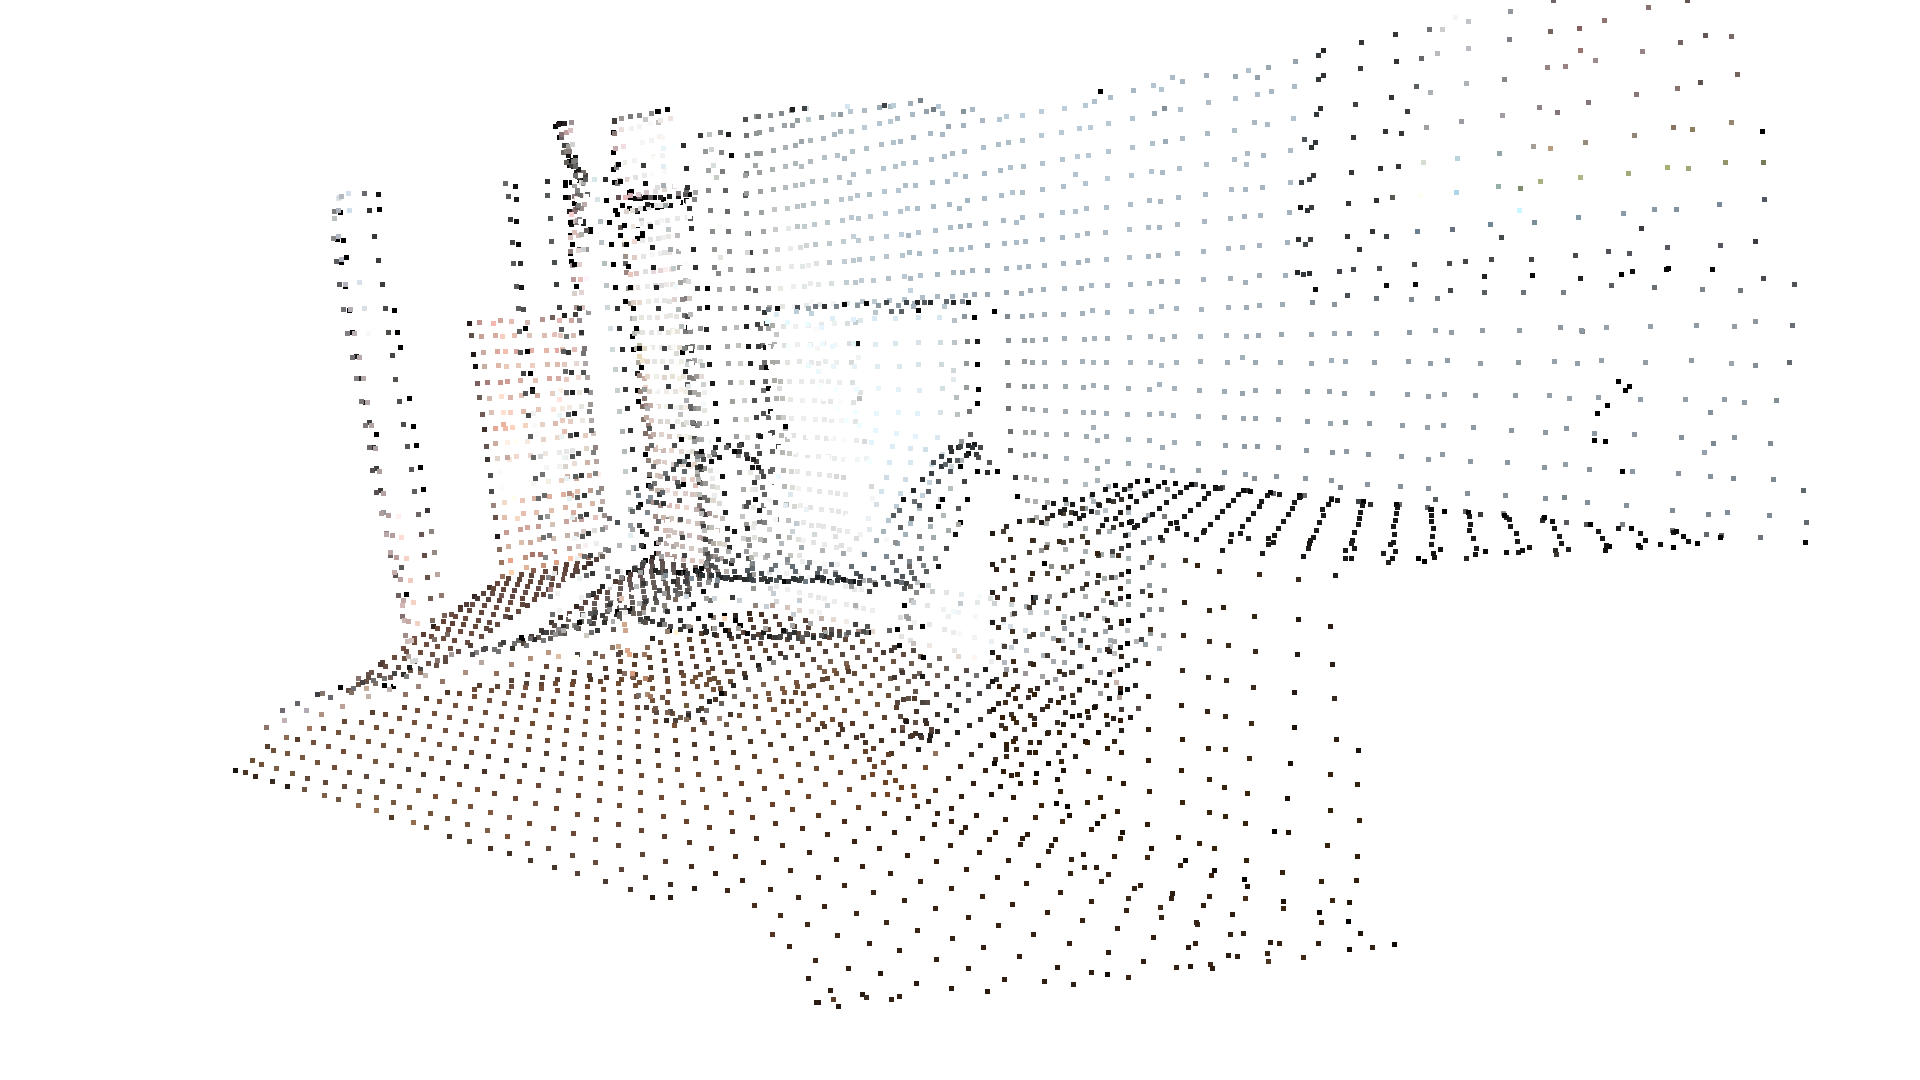
\includegraphics[ width=.5\textwidth ]{PointCloud}
    \caption{Beispiel einer drei-dimensionalen Point-Cloud-Rekonstruktion\label{fig:PointCloud}}\par
\end{figure}

\subsection{Bundle Adjustment}

Der Bundle Adjustment ist ein Optimierungsverfahren, das verwendet wird, um die Kamerapositionen und die 3D-Struktur der Szene zu verfeinern. Dabei werden die Fehler zwischen den projizierten 3D-Punkten und den tatsächlichen 2D-Punkten minimiert, um die bestmögliche Schätzung der Kamerapositionen und der 3D-Struktur zu erhalten. Der Bundle Adjustment ist ein iterativer Prozess, der normalerweise auf der nicht-linearen Optimierung basiert. Es gibt verschiedene Algorithmen zur Bundle Adjustment, wie z. B. die Levenberg-Marquardt-Methode oder die Gauss-Newton-Methode.

\section{SLAM}\label{SLAM}

Simultanous Localization and Mapping (SLAM) entstammt urprünglich aus der Robotik und beschreibt die Fähigkeit eines autonomen Systems, sich in einer unbekannten Umgebung zu lokalisieren und gleichzeitig eine Karte dieser Umgebung zu erstellen. SLAM ist sehr stark mit Structure-from-Motion-Algorithmen verwandt, da beide Techniken die gleichen Prinzipien verwenden, um die Kameraposition und die 3D-Struktur der Szene zu bestimmen. Der grundlegende Unterschied besteht darin, dass SLAM die Priorität auf die Echtzeitverarbeitung und die gleichzeitige Schätzung der Position und Orientierung des Sensors und die dreidimensionale Rekonstruktion der Umgebung legt. 

\section{Scene Understanding}

TODO

\section{Technische Limitationen}

Viele der gängigen Algorithmen zur Feature-Erkennung und -Verfolgung, wie SIFT oder ORB, verlassen sich stark auf die visuelle Qualität der Eingabebilder. In Umgebungen mit schlechten Lichtverhältnissen (z. B. bei schwacher Beleuchtung, direkter Sonneneinstrahlung oder Nachtaufnahmen) wird die Fähigkeit der Algorithmen zur präzisen Merkmalserkennung und -verfolgung beeinträchtigt. Dies kann zu fehlerhaften Schätzungen der Kameraposition oder der 3D-Rekonstruktion führen.

Ein weiteres Problem tritt auf, wenn sich die Umgebung schnell verändert, etwa bei Bewegungen von Objekten, plötzlichen Änderungen der Szene oder in dynamischen Umgebungen. In solchen Fällen können Feature-Punkte in den Bildern verschwinden oder durch neue, nicht korrespondierende Punkte ersetzt werden, was die Stabilität der Berechnungen negativ beeinflusst.

Auch LiDAR-basierte Systeme sind von technischen Einschränkungen betroffen. Zum einen haben LiDAR-Sensoren eine begrenzte Reichweite, die oft auf wenige Meter beschränkt ist, wodurch sie nicht für alle Anwendungen geeignet sind, insbesondere bei großen Distanzen oder in weiten offenen Bereichen.

Zudem sind LiDAR-Sensoren in der Regel teuer und daher nur vereinzelt in Smartphones verbaut. LiDAR-basierte Systeme sind vor allem in spezialisierten Bereichen wie der Automobilindustrie oder der Robotik weit verbreitet, aber in konsumerorientierten Geräten noch eher selten.